\documentclass[11pt, a4paper]{article}
\usepackage{fontspec} % Umlaute im eps sind nicht zusammengesetzt
\usepackage{lmodern} % Vektor-Schriftart
\usepackage{polyglossia}
\setmainlanguage{german}
\usepackage{graphicx} % Einbinden von Grafiken / SVG-Dateien moussen zuvor als eps exportiert werden
\usepackage{url} % Four URLs in der Bibliographie
\usepackage{amstext} % Four nichtkursiven Text in Formeln
\usepackage{listings}
\lstset{literate=%
	{Ö}{{\"O}}1
	{Ä}{{\"A}}1
	{Ü}{{\"U}}1
	{ß}{{\ss}}1
	{ü}{{\"u}}1
	{ä}{{\"a}}1
	{ö}{{\"o}}1
	{~}{{\textasciitilde}}1
}
\usepackage[dvipsnames]{xcolor}
\lstset{
	numbers= left,
	language=C++,
	keywordstyle=\color{Blue},
	stringstyle=\color{Orange},
	commentstyle=\color{OliveGreen},
	breaklines=true,
	extendedchars=true,
	basicstyle=\footnotesize\ttfamily,
	tabsize=4,
	frame=single,
	rulecolor=\color{black},
	captionpos=b,
	morekeywords={Vector3, Matrix, Transform, Vector4, Vector6,  EulerAngleXYZVector, Position, Vector, Rotation}}
\lstset{literate={-}{{-\allowbreak}}{1} }

\usepackage{etoolbox}% http://ctan.org/pkg/etoolbox
\makeatletter
\patchcmd{\lst@GLI@}% <command>
{\def\lst@firstline{#1\relax}}% <search>
{\def\lst@firstline{#1\relax}\def\lst@firstnumber{#1\relax}}% <replace>
{\typeout{listings firstnumber=firstline}}% <success>
{\typeout{listings firstnumber not set}}% <failure>
\makeatother
\newcommand{\code}{\texttt}
\usepackage{textcomp}
\usepackage{gensymb}
\usepackage{float}
\usepackage{csquotes}
\usepackage{amsmath}
%\usepackage{microtype}
\usepackage{tikz}
\date{\today}
\hyphenation{Trans-for-ma-ti-ons-ma-t-ri-zen, Trans-for-ma-ti-ons-ma-t-rix,Ko-or-di-na-ten-sys-teme,Ko-or-di-na-ten-sys-tem}
\begin{document}
\begin{center}
{\Huge Hochschule Darmstadt} \\
\vspace{0.5cm}
Lehrveranstaltung: Simulation von Robotersystemen \\
Prof. Dr. Thomas Horsch \\
Kalibrierung\\
Datum: 27.5.2016 \\
\vfill
\renewcommand{\arraystretch}{2}
	\begin{tabular}{| l | l |}
	\hline
	Name & Matrikelnummer \\ \hline
	Fabian Alexander Wilms & 735162 \\ \hline
	\end{tabular} \\
\vspace{0.5cm}
Studiengang: Mechatronik \\
Abgabedatum: 3.6.2016 \\
\vspace{0.5cm}
\begin{tabular}{| l | p{5cm} |}
	\hline
	Testat & \\ \hline
\end{tabular}
\renewcommand{\arraystretch}{1}
\end{center}
\newpage
\tableofcontents
\newpage
\section{Transformation zwischen zwei Koordinatensystemen}
Das Ziel dieser Aufgabe ist es, die Transformationsmatrix zwischen zwei Koordinatensystemen K0 und K1 zu bestimmen. Die beiden Koordinatensysteme sind durch jeweils 3 Punkte im Weltkoordinatensystem (KW) definiert: Den Ursprung (\code{K0o, K1o}), einen Punkt auf der positiven X-Achse (\code{K0x, K1x}) und einen Punkt auf der positiven Y-Achse (\code{K0y, K1y}). Die Z-Achse ist damit eindeutig bestimmt.

Durch Messungenauigkeiten kann es vorkommen, dass die jeweils 3 Punkte kein orthogonales Koordinatensystem bilden. Zudem haben die Punkte auf X- und Y-Achse nicht notwendigerweise den Abstand 1 vom Ursprung. Um aus diesen Punkten dennoch ein orthogonales Koordinatensystem zu erhalten, wird die Schmidtsche Orthonormalisierung angewendet.

Die neuen Vektoren $x$, $y$ und $z$ werden wie folgt berechnet:

\begin{eqnarray*}
x &=& \frac{X-Origin}{|X-Origin|} \\
b_2 &=& Y - Origin - \frac{(Y-Origin)^T \cdot (X-Origin)}{(X-Origin)^T \cdot (X-Origin)} \cdot (X- Origin) \\
y &=& \frac{b_2}{|b_2|} \\
z &=& x \times y
\end{eqnarray*}

Diese Orthonormalisierung wird für beide Koordinatensysteme durchgeführt, wodurch man für jedes orthogonale Koordinatensystem den Ursprung und die Vektoren x, y und z erhält.

Diese beiden Koordinatensysteme werden dann in jeweils eine Transformationsmatrix umgeformt, die den Übergang vom Weltkoordinatensystem nach K0 bzw. K1 beschreibt.

Die Transformationsmatrix $^{K0}T_{K1}$ kann daraufhin wie folgt bestimmt werden:

\begin{eqnarray*}
^{K0}T_{K1} = ^{K0}T_{KW} \cdot ^{KW}T_{K1} = (^{KW}T_{K0})^{-1} \cdot ^{KW}T_{K1}
\end{eqnarray*}

\lstinputlisting[firstline=18,lastline=85,caption={Transformation zwischen zwei Koordinatensystemen}]{../Termin4_1/Termin4_1.cpp}

Der Einfachheit halber wurde nicht mit realen Messpunkten getestet, sondern es wurden zwei Koordinatensysteme vorgegeben.

\begin{figure}[H]
\center\begin{tikzpicture}
\draw [->] (0,0) node {\hspace{-2em}$W_O$} -- node [pos=1] {\hspace{2em}$W_X$} (1,0);
\draw [->] (0,0) -- node [pos=1] {\hspace{-2em}$W_Y$} (0,1);

\draw [->] (1,2) node {\hspace{-2em}$K0_O$} -- node [pos=1] {\hspace{5em}$K0_X, K1_X$} (2,2);
\draw [->] (1,2) -- node [pos=1] {\hspace{-2em}$K0_Y$} (1,3);

\draw [->] (2,1) node {\hspace{2em}$K1_O$} -- (2,2);
\draw [->] (2,1) -- node [pos=1] {\hspace{-2em}$K1_Y$} (1,1);
\end{tikzpicture}
\caption{Die vorgegebenen Koordinatensysteme}
\end{figure}

\lstinputlisting[caption={Nicht orthogonale Messpunkte des ersten Koordinatensystems}]{../x86/Debug/4_1_System1.txt}

\lstinputlisting[caption={Nicht orthogonale Messpunkte des zweiten Koordinatensystems}]{../x86/Debug/4_1_System2.txt}

\lstinputlisting[caption={Ausgabe},keywords={}]{4-1.txt}

Es ergibt sich also folgende Transformationsmatrix:
\begin{equation*}
T = \begin{bmatrix}
0.010000    &    -0.999950   &    0.000000    &    0.990000 \\
0.999950    &    0.010000    &    0.000000    &    -1.000000 \\
0.000000    &    0.000000    &    1.000000    &    0.000000 \\
0.000000    &    0.000000    &    0.000000    &    1.000000
\end{bmatrix}
\end{equation*}
\newpage
\section{Verkettung von Transformationen}
Da der Arbeitsraum des MicroScribe-Gerätes begrenzt ist, benötigt man einen Weg, diesen zu erweitern. Dies ist möglich, indem man in Position 1 des Gerätes ein Koordinatensystem K0 vermisst, dann das Gerät an anderer Stelle platziert und die Messung desselben Koordinatensystems aus Position 2 wiederholt. Vermisst man nun ein zweites Koordinatensystem K1 von Position 2 aus, so lässt sich die Transformation relativ zu Position 1 berechnen, was eine Erweiterung des Arbeitsraumes bedeutet.

Man verkettet dieses Verfahren, indem man nun K2 von Position 2 und 3 aus misst, K3 von Position 3 und 4 usw. Sind das erste und das letzte gemessene Koordinatensystem dasselbe, so muss das Produkt der einzelnen Transformationsmatrizen idealerweise gleich der Einheitsmatrix sein: 
\begin{eqnarray*}
K0 \cdot \sum_i^n{^iT_{i+1}} = K0 \cdot E = K0
\end{eqnarray*}
Der Algorithmus aus Aufgabe 1 wird in eine Funktion integriert:
\lstinputlisting[firstline=16,lastline=66,caption={Transformation zwischen zwei Koordinatensystemen}]{../Termin4_2/Termin4_2.cpp}

\lstinputlisting[firstline=79,lastline=106,caption={Verkettung von Transformationen}]{../Termin4_2/Termin4_2.cpp}

Getestet wurde der Algorithmus mit 8 vorgegebenen Transformationsmatrizen:
\lstinputlisting[caption={Ausgabe},keywords={}]{4-2.txt}
Die aus der Verkettung der Transformationen resultierende Matrix
\begin{equation*}
T_{Ist} = \begin{bmatrix}
0.999905    &    -0.012206   &    0.006358    &    -1.205218 \\
0.012191    &    0.999923    &    0.002337    &    1.215314 \\
-0.006386   &    -0.002259   &    0.999977    &    -0.128655 \\
0.000000    &    0.000000    &    0.000000    &    1.000000
\end{bmatrix}
\end{equation*}
entspricht annähernd genau der idealen Lösung (d.h. Einheitsmatrix) $T_{Soll}$
\begin{equation*}
T_{Soll} = \begin{bmatrix}
1.000000    &    0.000000    &    0.000000   &     0.000000 \\
0.000000    &    1.000000    &    0.000000   &     0.000000 \\
0.000000    &    0.000000    &    1.000000   &     0.000000 \\
0.000000    &    0.000000    &    0.000000   &     1.000000
\end{bmatrix}
\end{equation*}
\newpage
\section{Kalibrierung}
Wird an einem Roboter ein Werkzeug angebracht, muss die Transformation vom alten zum neuen TCP bestimmt werden. Da die neue Messspitze parallel zur ursprünglichen verläuft, enthält die Transformation keine Rotation, sondern nur den Translationsvektor $P_t$.

Um diesen zu bestimmen sucht man sich einen festen Punkt $P_{pivot}$ im Weltkoordinatensystem, dessen Koordinaten nicht bekannt sein müssen und fährt mit dem Roboter verschiedene Posen an, wobei immer die Position des neuen TCP identisch zu $P_{pivot}$ sein muss (dies nennt sich \enquote{Quirlen}).

Da der direkte Weg zum Drehpunkt $P_{pivot}$ mit dem indirekten über $P_i$ und anschließend $R_i \cdot P_t$ identisch sein soll muss gelten:

\begin{equation*}
P_i + R_i \cdot P_t - P_{pivot} \cong 0
\end{equation*}
 mit $i = 1..n$.

Bringt man $P_i$ auf die rechte Seite und drückt $R_i \cdot P_t - P_{pivot}$ durch eine Matrixmultiplikation aus, so erhält man

\begin{eqnarray*}
&\underbrace{
\begin{pmatrix}
R_1 & -I \\ \vdots & \vdots \\ R_n & -I
\end{pmatrix}}_{\textnormal{Koeffizientenmatrix A}} \cdot
\underbrace{
\begin{pmatrix}
P_t \\ P_{pivot}
\end{pmatrix}}_{\textnormal{Parameter x}}
\cong
\underbrace{
\begin{pmatrix}
-P_1 \\ \vdots \\ -P_n
\end{pmatrix}}_{\textnormal{Beobachtungen b}}\\
\Leftrightarrow & A \cdot x \cong b
\end{eqnarray*}

Da die Messungen fehlerbehaftet sind, muss auf der rechten Seite der Residuenvektor $r$ hinzu addiert werden, welcher die Fehler kompensiert.

\begin{equation*}
A \cdot x = b + r
\end{equation*}

Gesucht sind jetzt die Werte für $P_t$ und $P_{pivot}$, für die der Fehler $r^T \cdot r$ minimal wird.

Dafür stellt man obige Gleichung nach r um, differenziert $r^T \cdot r$ nach x und setzt dies gleich 0. Daraus ergibt sich

\begin{equation}
x = (A^T \cdot A)^{-1} \cdot A^T \cdot b
\end{equation}

Da es 6 Unbekannt gibt, werden auch mindestens 2 Messposen benötigt, um das Gleichungssystem lösen zu können.

\begin{figure}[H]
	\centering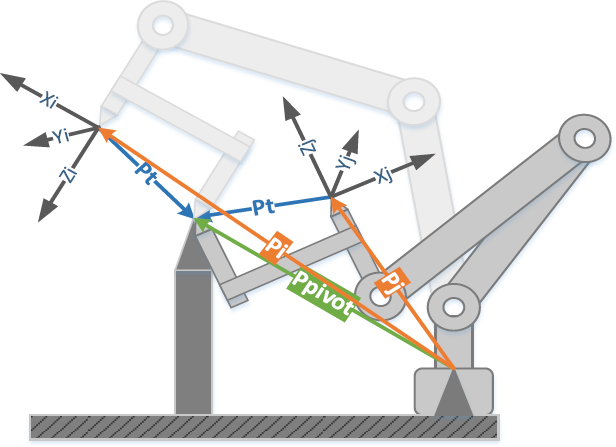
\includegraphics[width=0.75\textwidth]{Quirlen.png}
	\caption{„Quirlen“ um einen festen Punkt im Raum}
\end{figure}

Die für $P_t$ und $P_{pivot}$ berechneten Werte lassen sich validieren, indem man den direkten Weg zum Drehpunkt $P_{pivot}$ mit dem indirekten über $P_i$ und anschließend $R_i \cdot P_t$ vergleicht. Idealerweise ist die Differenz $\vec{0}$.

\begin{equation}
P_{test} = R_i \cdot P_t + P_i - P_{pivot} \overset{!}{=} \vec{0}
\end{equation}

Der folgende Algorithmus extrahiert zunächst für jeden gemessenen Frame die Position und die Rotation des ursprünglichen TCP und baut daraus die Matrix A sowie den Vektor b auf. Anschließend wird Gleichung (1) angewendet und die berechneten Werte für $P_t$ und $P_{pivot}$ mit Gleichung (2) validiert. Zum Validieren muss wieder für jeden Frame Rotation und Position extrahiert werden, um sie in die Gleichung einsetzen zu können.

Zuletzt wird die Standardabweichung des Ergebnisses mit folgender Formel bestimmt:

\begin{equation*}
s_0=\sqrt{\frac{r^T \cdot r}{n}}
\end{equation*}

\lstinputlisting[firstline=22,lastline=96,caption={Kalibrierung}]{../Termin4_3/Termin4_3.cpp}

$P_{test}$ wurde für jede in \code{Kreisel.txt} enthaltene Messpose berechnet:

\lstinputlisting[firstline=1,lastline=23,caption={Ausgabe},keywords={}]{4-3.txt}

\lstinputlisting[firstline=75,lastline=81,caption={Ausgabe},keywords={}]{4-3.txt}

Wie erwartet gilt für jede Messpose $P_{test} \approx \vec{0}$.
\end{document}